% VUT FIT MITAI
% MSZ 2021/2022
% Author: Vladimir Dusek
% Login: xdusek27

%%%%%%%%%%%%%%%%%%%%%%%%%%%%%%%%%%%%%%%%%%%%%%%%%%%%%%%%%%%%%%%%%%%%%%%%%%%%%%%%

% Path to figures
\graphicspath{{tin/slozitost/figures}}

%%%%%%%%%%%%%%%%%%%%%%%%%%%%%%%%%%%%%%%%%%%%%%%%%%%%%%%%%%%%%%%%%%%%%%%%%%%%%%%%

\chapter{TIN~--~Časová a paměťová složitost (třídy složitosti, úplnost, SAT problém).}

%%%%%%%%%%%%%%%%%%%%%%%%%%%%%%%%%%%%%%%%%%%%%%%%%%%%%%%%%%%%%%%%%%%%%%%%%%%%%%%%

\section{Zdroje}

\begin{compactitem}
    \item \path{tin_2021_merged.pdf}
    \item \path{TIN_2020-12-01.mp4}
    \item \path{TIN_2020-12-04_demo.mp4}
    \item \path{TIN_2020-12-08.mp4}
    \item \path{TIN_2020-12-11_demo.mp4}
\end{compactitem}

%%%%%%%%%%%%%%%%%%%%%%%%%%%%%%%%%%%%%%%%%%%%%%%%%%%%%%%%%%%%%%%%%%%%%%%%%%%%%%%%

\section{Úvod a kontext}

% složitost problému vs složitost algoritmu ?

% Co je to NP-úplnost, co je obecně úplnost a těžkost.

% Chtěl slyšet příklad nějakého NP-úplného problému. Když jsem řekl SAT, tak chtěl definovat, co je to SAT problém.

\begin{compactitem}
    \item Časová složitost -- počet kroků (přechodů) TS provedený od počátku do konce výpočtu.

    \item Prostorová (paměťová) složitost -- počet buněk pásky TS požadovaný pro daný výpočet.

    \item Je-li časová složitost výpočtu prováděného TS rovna $n$, pak prostorová složitost tohoto výpočtu není větší než $n + 1$. \begin{compactitem}
        \item Tvrzení je jednoduchou implikací plynoucí z definice časové a prostorové složitosti.
    \end{compactitem}

    \item Při popisu složitosti algoritmů (výpočtů TS), chceme často vyloučit vliv aditivních a multiplikativních konstant: \begin{compactitem}
        \item Různé aditivní a multiplikativní konstanty vzniknou velmi snadno \uv{drobnými} úpravami uvažovaných algoritmů.
        \item Primárně nás zajímá, jak složitost roste v závislosti na délce vstupu. Zejméne pro dlouhé vstupy.
    \end{compactitem}

    \item Různé případy při analýze složitosti: \begin{compactitem}
        \item analýza složitosti nejhoršího případu,
        \item analýza složitosti nejlepšího případu,
        \item analýza složitosti průměrného případu,
        \item amortizovaná analýza -- Studuje posloupnost operací jako celek. Tato technika umožňuje, na rozdíl od klasického přístupu mnohem přesnější určení časové složitosti algoritmu.
    \end{compactitem}

\end{compactitem}

%%%%%%%%%%%%%%%%%%%%%%%%%%%%%%%%%%%%%%%%%%%%%%%%%%%%%%%%%%%%%%%%%%%%%%%%%%%%%%%%

\section{Asymptotická složitost}

\begin{compactitem}
    \item Složitost algoritmů, resp. turingových strojů.

    \item Asymptotická složitost -- neřešíme aditivní a multiplikativní konstanty a bereme v potaz pouze nejvyšší polynom.

    \item Nechť $\mathcal{F}$ je množina funkcí $f : \mathbb{N} \rightarrow \mathbb{N}$. Pro danou funkci $f \in \mathcal{F}$ definujeme množiny funkcí $\mathcal{O}(f(n))$, $\Omega(f(n))$ a $\Theta(f(n))$ následovně: \begin{compactitem}

        \item \textbf{Asymptotické horní omezení} funkce $f(n)$ je množina
        $$ \mathcal{O}(f(n)) = \{ g(n) \in \mathcal{F} ~|~ \exists c \in \mathbb{R}^{+} ~\exists n_0 \in \mathbb{N} ~\forall n \in \mathbb{N} : n \geq n_0 : 0 \leq g(n) \leq c \cdot f(n) \} $$

        \item \textbf{Asymptotické dolní omezení} funkce $f(n)$ je množina
        $$ \Omega(f(n)) = \{ g(n) \in \mathcal{F} ~|~ \exists c \in \mathbb{R}^{+} ~\exists n_0 \in \mathbb{N} ~\forall n \in \mathbb{N} : n \geq n_0 : 0 \leq c \cdot f(n) \leq g(n) \} $$

        \item \textbf{Asymptotické oboustranné omezení} funkce $f(n)$ je množina
        $$ \Theta(f(n)) = \{ g(n) \in \mathcal{F} ~|~ \exists c_1, c_2 \in \mathbb{R}^{+} ~\exists n_0 \in \mathbb{N} ~\forall n \in \mathbb{N} : n \geq n_0 : $$
        $$ : 0 \leq c_1 \cdot f(n) \leq g(n) \leq c_2 \cdot f(n) \} $$

    \end{compactitem}
\end{compactitem}

\begin{figure}[H]
    \centering
    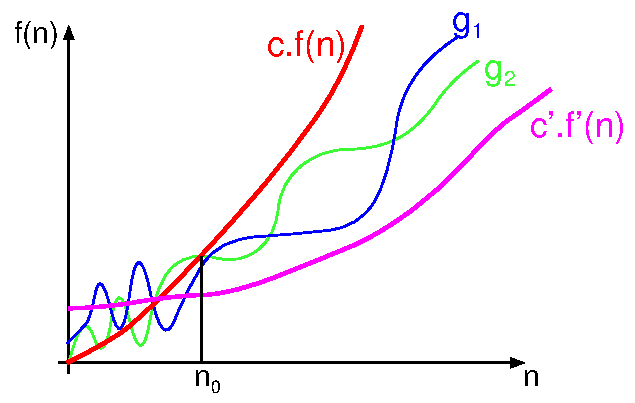
\includegraphics[width=0.75\linewidth]{complexity.pdf}
    \caption{Asymptotická složitost.}
\end{figure}

%%%%%%%%%%%%%%%%%%%%%%%%%%%%%%%%%%%%%%%%%%%%%%%%%%%%%%%%%%%%%%%%%%%%%%%%%%%%%%%%

\section{Třídy složitosti}

\begin{compactitem}
    \item Složitosti problémů.

    \item Třídy složitosti zavádíme jako prostředek ke kategorizaci (vytvoření hierarchie) problémů dle jejich složitosti, tedy dle toho, jak dalece efektivní algoritmy můžeme navrhnout pro jejich rozhodování.

    \item Mějme dány funkce $t, s : \mathbb{N} \rightarrow \mathbb{N}$ a nechť $T_M$, resp. $S_M$, značí časovou, resp. prostorovou, složitost TS $M$. Definujeme následující časové a prostorové třídy složitosti deterministických a nedeterministických TS:
    $$DTime[ t(n) ] = \{ L ~|~ \exists k \text{-páskový DTS } M : L = L(M) ~\land~ T_M \in \mathcal{O}(t(n)) \}$$

    $$NTime[ t(n) ] = \{ L ~|~ \exists k \text{-páskový NTS } M : L = L(M) ~\land~ T_M \in \mathcal{O}(t(n)) \}$$

    $$DSpace[ s(n) ] = \{ L ~|~ \exists k \text{-páskový DTS } M : L = L(M) ~\land~ S_M \in \mathcal{O}(s(n)) \}$$

    $$NSpace[ s(n) ] = \{ L ~|~ \exists k \text{-páskový NTS } M : L = L(M) ~\land~ S_M \in \mathcal{O}(s(n)) \}$$

    \item Definici tříd složitosti pak přímočaře zobecňujeme tak, aby mohly být založeny na množině funkcí, nejen na jedné konkrétní funkci.

    \item Modely turingova stroje a vyčíslitelnost/složitost: \begin{compactitem}

        \item Nedeterminismus nepřináší nic z pohledu vyčíslitelnosti. Z pohledu složitosti, lze NTS lze implementovat deterministickým TS, ale za cenu exponenciálního nárůstu času.

        \item Více pásek nepřináší nic z pohledu vyčíslitelnosti. Z pohledu složitosti přináší více pásek polynomiální zrychlení.

    \end{compactitem}
\end{compactitem}

\paragraph*{Deterministický/nedeterministický polynomiální čas} $$ \mathbf{P} = \bigcup_{k=0}^{\infty} DTime(n^k) ~~~~~ \equiv^? ~~~~~ \mathbf{NP} = \bigcup_{k=0}^{\infty} NTime(n^k) $$

\paragraph*{Deterministický/nedeterministický polynomiální prostor} $$ \mathbf{PSPACE} = \bigcup_{k=0}^{\infty} DSpace(n^k) ~~~~~ \equiv ~~~~~ \mathbf{NPSPACE} = \bigcup_{k=0}^{\infty} NSpace(n^k) $$

\paragraph*{Deterministický/nedeterministický logaritmický prostor} $$ \mathbf{LOGSPACE} = \bigcup_{k=0}^{\infty} DSpace(k \cdot \log(n)) ~~~~~ \equiv^? ~~~~~ \mathbf{NLOGSPACE} = \bigcup_{k=0}^{\infty} NSpace(k \cdot \log(n)) $$

\paragraph*{Deterministický/nedeterministický exponenciální čas} $$ \mathbf{EXP} = \bigcup_{k=0}^{\infty} DTime(2^{n^k}) ~~~~~ \equiv^? ~~~~~ \mathbf{NEXP} = \bigcup_{k=0}^{\infty} NTime(2^{n^k}) $$

\paragraph*{Deterministický/nedeterministický exponenciální prostor} $$ \mathbf{EXPSPACE} = \bigcup_{k=0}^{\infty} DSpace(2^{n^k}) ~~~~~ \equiv ~~~~~ \mathbf{NEXPSPACE} = \bigcup_{k=0}^{\infty} NSpace(2^{n^k}) $$
